\chapter{Related work}
This chapter explains the necessary basis to understand the procedure and contains all relevant information of previous work in this field.

\section{Artificial neural networks}

% \section{} MLP?

\glspl{ann} have become the de facto standard in image classification.%cite 
The main architectures are \glspl{cnn} and the more recent \glspl{vit}.

\subsection{Convolutional neural networks}
Dense neural networks are not suited for images. A $224$ pixel high and $244$ pixel wide image would require millions of parameters per layer, which is not feasible. But it is not necessary to regard all pixel in every neuron of the following layer. 
Pixels highly correlate with their adjacent neighbours and contain redundancy. 
Filters combine pixels locally to extract meaningful features per region. Occasional pooling layers scale down the layer size and reduce the number of required neurons greatly. The reduction of values also enables the succeeding filters to combine the local features more and more until the linear classification layer.

% Images are very sparse data.
% The main idea of \glspls{cnn} is the use of convolutional layers to greatly reduce the number of neurons 
% Normal downscaling would lose important details. 
% Number of Maps
% Number of linear nodes/parameters

\begin{figure}[H]
    \begin{center}
    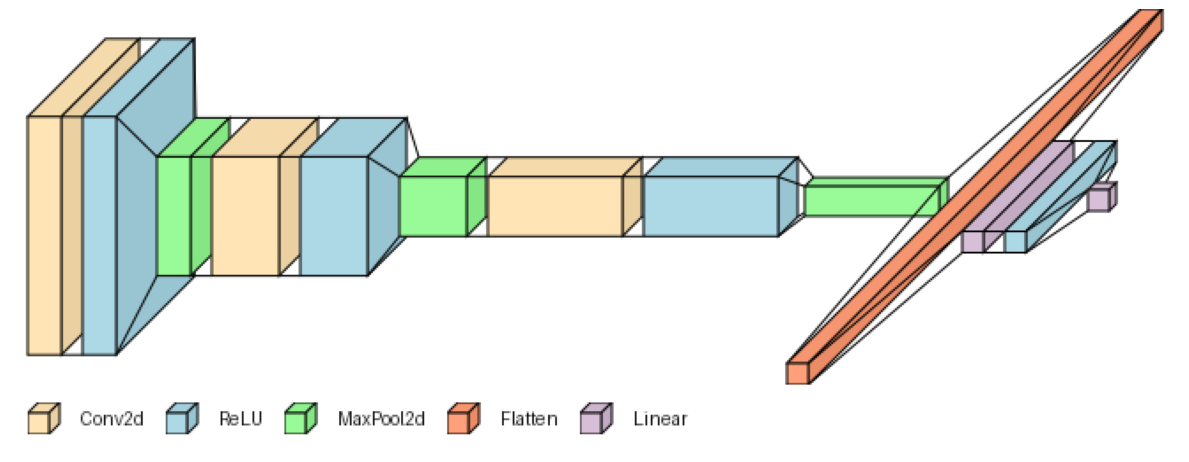
\includegraphics[width=15cm]{../images/cnn_architecture.png}
    \caption{Architecture of a basic \gls{cnn}}\label{fig:cnn_architecture}
    \end{center}
\end{figure}

An example of a \gls{cnn} is shown in Figure~\ref{fig:cnn_architecture}. The images is fed into the network on the left side. The convolutional layers increase the number of stacked maps, visualized by wider layers. The pooling layers decrease the height and width. The flattening concatenates all datapoints into a one-dimensional vector. This vector can then be used by dense layers to decrease the number of nodes to the number of classes.

% \section{Models}

\subsection{Resnet50}
Figure~\ref{fig:resnet50_architecture}.

\begin{figure}[H]
    \begin{center}
    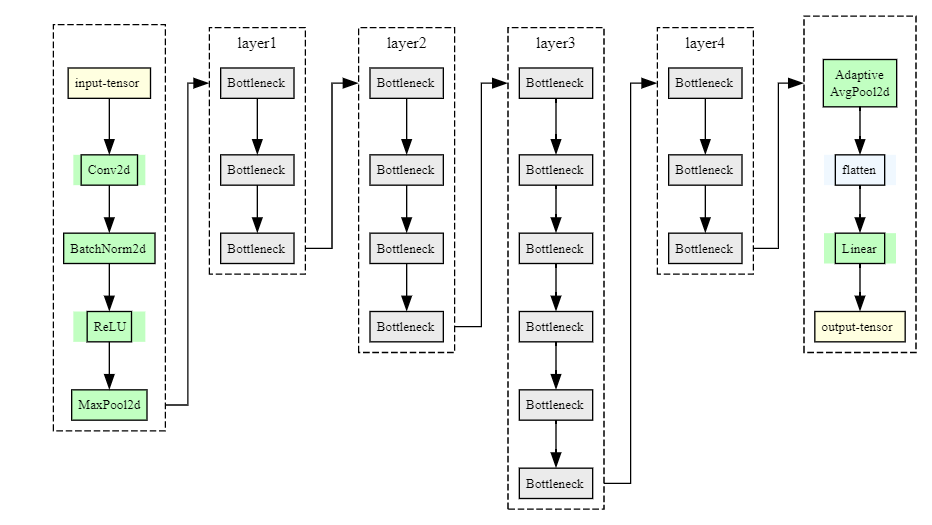
\includegraphics[width=15cm]{../images/resnet50_architecture.png}
    \caption{Architecture of Resnet50}\label{fig:resnet50_architecture}
    \end{center}
\end{figure}

Figure~\ref{fig:resnet50_architecture_bottleneck}.

\begin{figure}[H]
    \begin{center}
    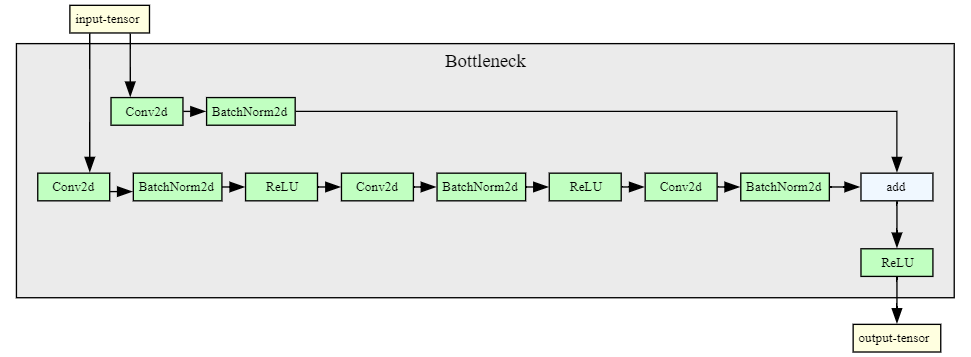
\includegraphics[width=15cm]{../images/resnet50_architecture_bottleneck.png}
    \caption{Architecture of Resnet50 bottleneck}\label{fig:resnet50_architecture_bottleneck}
    \end{center}
\end{figure}

\subsection{ViT-T/16}
Figure~\ref{fig:vit_t16_architecture}.

\begin{figure}[H]
    \begin{center}
    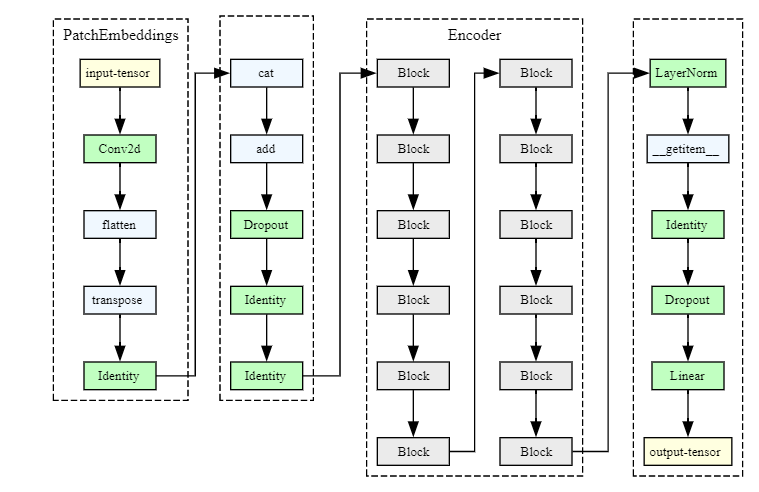
\includegraphics[width=15cm]{../images/vit_t16_architecture.png}
    \caption{Architecture of ViT-T/16}\label{fig:vit_t16_architecture}
    \end{center}
\end{figure}

Figure~\ref{fig:vit_t16_architecture_block}.

\begin{figure}[H]
    \begin{center}
    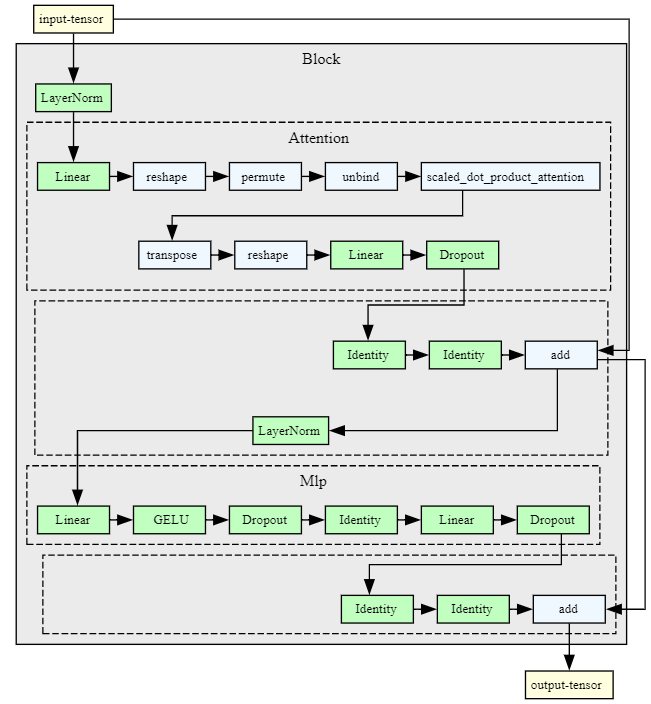
\includegraphics[width=15cm]{../images/vit_t16_architecture_block.png}
    \caption{Architecture of ViT-T/16 block}\label{fig:vit_t16_architecture_block}
    \end{center}
\end{figure}


% AI
% Finetuning / Transfer Learning
% Modern approaches: Lora, Adapter
% Frozen evaluation
% Utility Score



% DINO
% Teacher / Student
